\chapter{Results} \label{chap:results}

In this chapter, we talk about the results. We start of by talking about the results achieved with different parameters during implementation and which we decided to use in the end. We then proceed to evaluate

\section{Implementation parameters}

\subsection{Storing moments} \label{sec:storingMoments}

The first thing we analyze is the technique used for storage and subsequent reconstruction of the Fourier coefficients. Specifically, we need to decide how to map wavelengths to a signal from which the coefficients are obtained. As already mentioned in~\cref{par:spectrumToCoefficientConversion}, we have the choice of both \emph{mirroring} and \emph{warping} the signal, which overall creates four options --- using only mirroring, using only warping, using both or using neither, i.e. utilizing the original signal.

To decide which of these options suits our problem the best, we run an experiment in which we compare the original color of a spectral curve with the color of a spectrum obtained by reconstruction from the original curve's coefficients. We use entries from multiple color atlases (such as the Pantone atlas, Munsell Book of Colors and Macbeth Color Checker) and we compute the average and maximum color difference. For these purposes, we use the Delta E error specified in~\cref{deltaE}. Although we state that the Delta 2000 is better, it is not(why? MFO) due to  discontinuities when using gradients

In~\cref{sec:completeMomentError}, we provide all results obtained from these experiments. Note that using $n$ moments requires storing $n+1$ values in case mirroring is used (i.e. the moments are real) and $2n+1$ values otherwise (i.e. the moments are complex). As we are interested in the number of $coefficients$ needed for storage (and for passing to the optimizer) rather than the number of moments, we surmise the contents of~\cref{sec:completeMomentError} in~\cref{table:comparisonMomentTechnique}, where we present the errors according to the number of coefficients.

\begin{table}[t]
	\centering
	\begin{tabular}{crrrrrrrr}
		\toprule
		\multirow{4}{*}{Coefficients} &
		\multicolumn{8}{c}{Methods} \\
		\cmidrule(lr){2-9}
		&\multicolumn{2}{c}{M\&W} &
		\multicolumn{2}{c}{M\&nW} &
		\multicolumn{2}{c}{nM\&W} &
		\multicolumn{2}{c}{nM\&nW}\\
		\cmidrule(lr){2-9}
		& Avg & Max & Avg & Max & Avg & Max & Avg & Max \\
		\cmidrule(lr){1-9}
		1&35.87&114.04&36.2&113.86&35.92&113.97&36.2&113.86\\
		2&21.3&91.19&26.4&99.44&\textemdash&\textemdash&\textemdash&\textemdash\\
		3&1.65&15.09&15.43&68.06&6.54&42.93&13.24&60.23\\
		4&0.86&5.6&9.93&55.67&\textemdash&\textemdash&\textemdash&\textemdash\\
		5&0.54&2.98&4.19&23.53&2.13&17.51&3.7&17.5\\
		6&0.34&2.22&1.19&5.68&\textemdash&\textemdash&\textemdash&\textemdash\\
		7&0.29&2.17&0.77&2.38&1.13&6.87&0.95&5.3\\
		8&0.28&2.03&0.77&1.86&\textemdash&\textemdash&\textemdash&\textemdash\\
		9&0.26&1.95&0.62&1.43&0.97&4.35&0.48&1.96\\
		\bottomrule
	\end{tabular}
	\caption{The average and maximum \emph{Delta E} error originating from round-trips, i.e. from converting spectra to coefficients $c$ and its subsequent reconstruction from $c$. $M$ represents mirroring, $W$ warping, and the symbol $n$ stands for their negation.}
	\label{table:comparisonMomentTechnique}
\end{table}

According to the observation of~\cref{table:comparisonMomentTechnique}, it is clearly beneficial to use mirroring. Choosing whether to warp the signal is slightly more complicated --- warping definitely performs better if the number of coefficients is below six (as a matter of fact, this is exactly the same conclusion that~\citet{trigonometricMomentsPresentation} has arrived to), and on average outperforms the non-warping strategy even when using higher number of coefficients. We, however, require successful round-trips only when fitting atlas lattice points, as the regular points do not have a prior atlas entry that their spectra must approximate. We therefore focus exclusively on the performance of these technique under 9 coefficients, as that is the number we use for fitting such entries. 

\begin{figure}[t]
	\centering
	\captionsetup[subfigure]{font=footnotesize,labelfont=footnotesize}
	\captionsetup[subfigure]{justification=centering}
	\begin{subfigure}[t]{0.60\textwidth}
		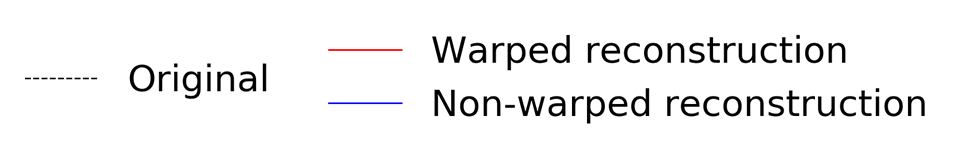
\includegraphics[width=\linewidth]{img/results_techniqueLegend.png}
	\end{subfigure} \\
	\begin{subfigure}[t]{0.45\textwidth}
		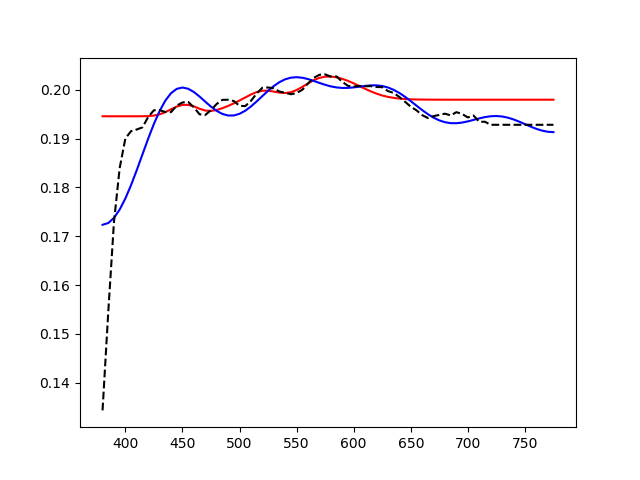
\includegraphics[width=\linewidth]{img/results_techniqueNeutral5.png}
		\caption{``neutral 5'' patch}
		\label{fig:resultsTechnique_neutral5}
	\end{subfigure} \hspace{0.1em}
	\begin{subfigure}[t]{0.45\textwidth}
		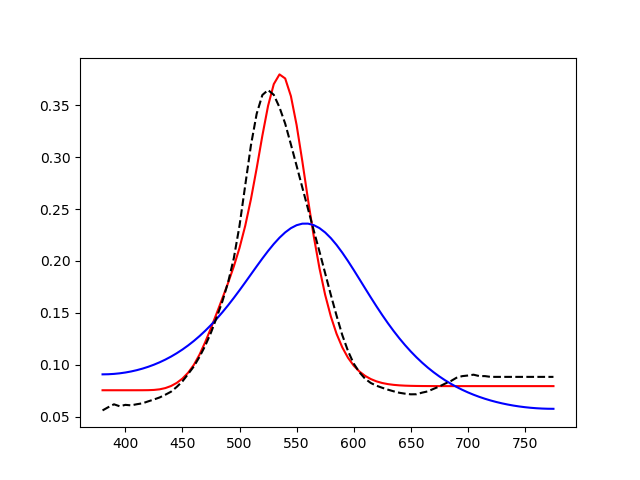
\includegraphics[width=\linewidth]{img/results_techniqueGreen.png}
		\caption{``green'' patch}
		\label{fig:resultsTechnique_green}
	\end{subfigure} \hspace{0.1em}
	\vspace{0.5em}\\
	\begin{subfigure}[t]{0.45\textwidth}
		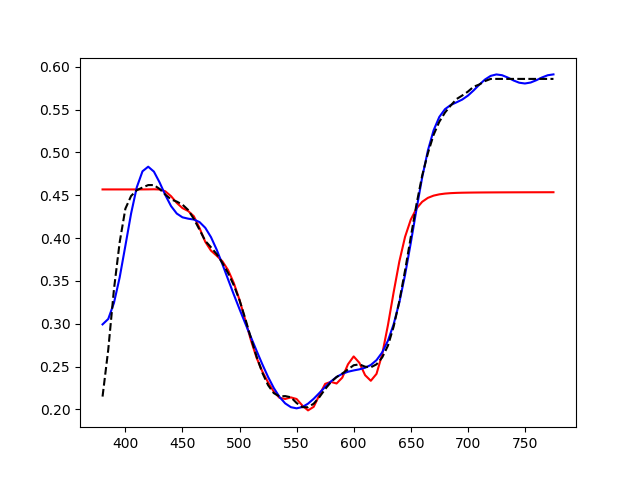
\includegraphics[width=\linewidth]{img/results_techniqueBlueFlower.png}
		\caption{``blue flower'' patch}
		\label{fig:resultsTechnique_blueFlower}
	\end{subfigure} \hspace{0.1em}
	\begin{subfigure}[t]{0.45\textwidth}
		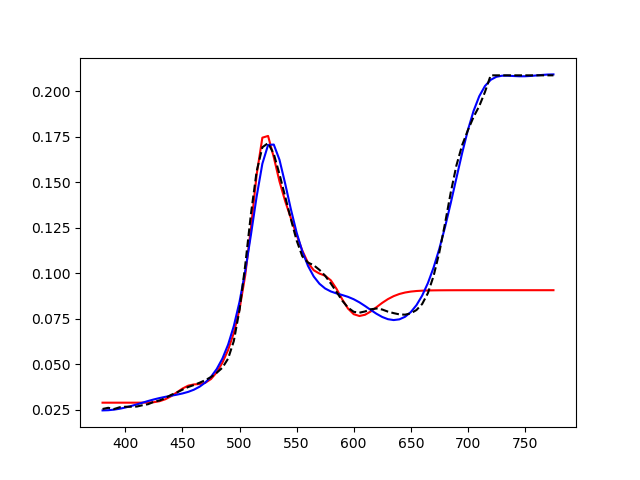
\includegraphics[width=\linewidth]{img/results_techniqueFoliage.png}
		\caption{``foliage'' patch}
		\label{fig:resultsTechnique_foliage}
	\end{subfigure}
	\caption{Comparison between the warped and non-warped reconstructed signal shown on multiple patches of the Macbeth Color Chart}
	\label{fig:resultsTechniques}
\end{figure}

In~\cref{fig:resultsTechniques}, we compare the techniques on a few patches of the Macbeth Color Chart by performing round-trips with 9 coefficients. The difference between the two methods is as mentioned in~\citet{trigonometricMomentsPaper} --- since warping focuses on the more important regions of the spectrum in terms of color perception (i.e. around 550nm), it reconstructs the slight waves in this area quite precisely while neglecting the edges. Non-warping, on the other hand, focuses on the spectra as a whole, which results in approximating the shape over the whole wavelength range but not in an exact replication of any specific spikes.

We cannot definitely determine the more precise method (e.g. warping gives the impression of better performance in case of the ``neutral 5'' patch in~\cref{fig:resultsTechnique_neutral5}, but seems to rather unsuccessful in the case of the ``blue flower'' patch in~\cref{fig:resultsTechnique_blueFlower}). However, the last row of~\cref{table:comparisonMomentTechnique} suggest that although warping performs better on average, its maximum achieved error is higher than that of the non-warping technique.

\begin{figure}[t]
	\centering
	\vspace{1em}
	\begin{subfigure}[t]{0.49\textwidth}
		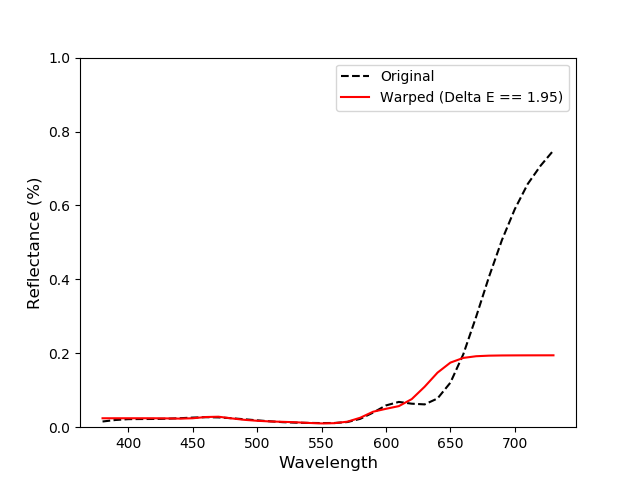
\includegraphics[width=\linewidth]{img/results_worstWarped.png}
		\caption{Warped spectral reconstruction of the Munsell 2.5R 2/6 sample from the Munsell Book of Color, Delta E == 1.95}
		\label{fig:resultWorstWarp}
	\end{subfigure} \hspace{0.1em}
	\begin{subfigure}[t]{0.49\textwidth}
		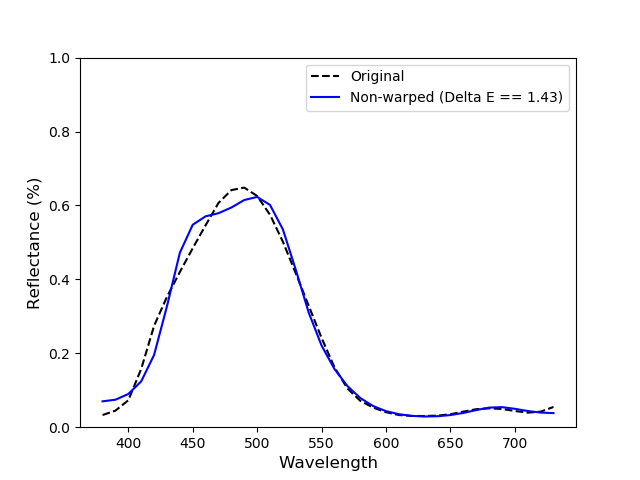
\includegraphics[width=\linewidth]{img/results_worstNonWarped.png}
		\caption{Non-warped spectral reconstruction of the Pantone 3551 C sample of the Pantone color atlas, Delta E == 1.43}
		\label{fig:resultWorstNonWarp}
	\end{subfigure}
	\caption{The worst-case round-trip scenarios of the warped and non-warped technique, 9 coefficients used for spectral reconstruction}
	\label{fig:resultsTechniquesWorst}
\end{figure}

The impact of the worst-case scenario on rendering is another important factor to consider in our decision-making process. Having even one incorrect color could cause significant metameric artifacts, which we want to avoid at all costs. Therefore, we specifically analyze the cases in which the maximum error was obtained. For warping, this represents the Munsell 2.5R 2/6 sample of the Munsell Book of Color, while non-warping performs worst for the Pantone 3551 C sample of the Pantone color atlas. We show the round-trip results of both of these cases in~\cref{fig:resultsTechniquesWorst}.

Although the shortcomings of warping can already be perceived in e.g.~\cref{fig:resultsTechnique_foliage} or~\cref{fig:resultsTechnique_blueFlower}, the failure in the reconstruction of the curve's edges does not have a significant effect of the the resulting RGB color, as the source of color is mainly focused around the middle of the curve. However, if the edges are extremely distinct from the rest of the curve (see~\cref{fig:resultWorstWarp}), they tend to provide unanticipated color information. In such cases, warping the signal presents a disadvantage.

Obviously, the Delta E error caused by unnecessary warping can be reduced to almost 0 by passing the computed coefficients to the optimizer, which then alters the curve so that it evaluates to the correct RGB. However, because we lose the notion of the curve's desired shape and because warping does not focus on the edges, the optimizer is apt to amplify the already existing slight bumps in the middle. This behavior may therefore cause the resulting shape to be extremely distinct from the desired one. 

The non-warping technique, shown in~\cref{fig:resultWorstNonWarp}, is not susceptible to this kind of behavior. Although it creates a rather significant Delta E error, we can observe that the shape of the reconstructed spectrum roughly resembles the original shape. Such a behavior is desired in our case, as the reconstructed reflectance is less prone to cause metameric artifacts under different illuminants. Additionally, as the non-warping technique forces the optimizer to not prioritize specific parts of the curve, the optimization is prone to slightly altering the shape as a whole rather than creating 
irregularities in the middle. Therefore, regardless of the average error, we assume the non-warping technique to outperform warping both when performing simple round-trips, but also if we use this method during the optimization process of fitting the cube.

We put our theory to test. We create a few cubes with varying parameters and we try to fit their entries with both techniques, using the cost functions determined in~\cref{ssec:costFunctions}. We present some of the results in~\cref{fig:resultsTechnique_optimizer}, but we examine many more spectra just to confirm our hypothesis. 

We conclude that our theory is correct --- warping indeed amplifies the slight differences around the middle of the curve in order to achieve the correct color, so much that it creates spikier spectra the more the cube grows. Although this does not necessarily render the cubes created with warped signal useless, it is apparent they are prone to creating memateric artifacts such as the ones presented in~\cref{fig:metamerism}. Additionally, as we already mentioned in ref, the interpolation phase of the rendering pipeline benefits from smooth, non-spiky spectra, which is a criterion the warped spectra do not satisfy. Therefore, we it is save to discard the option of warping.

\begin{figure}[t]
	\centering
	\captionsetup[subfigure]{font=footnotesize,labelfont=footnotesize}
	\captionsetup[subfigure]{justification=centering}
	\begin{subfigure}[t]{0.38\textwidth}
		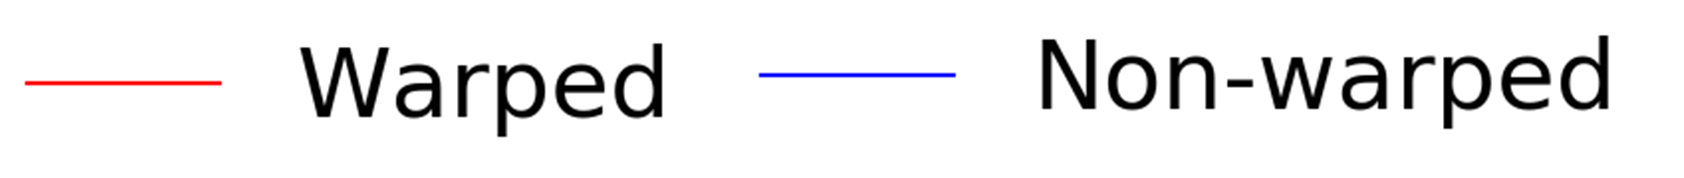
\includegraphics[width=\linewidth]{img/resultsTechniqueOpt_legend.png}
	\end{subfigure} \\
	\begin{subfigure}[t]{0.31\textwidth}
		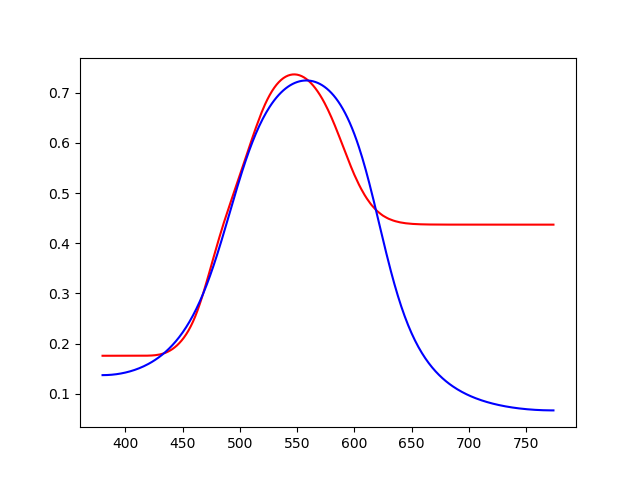
\includegraphics[width=\linewidth]{img/resultsTechniqueOpt_m3_cd64.png}
		\caption{$c=3, cd=64$,\\$RGB=(222.6, 230.7, 230.7)$,\\initial atlas = Macbeth Color Chart}
		\label{fig:resultsTechniqueOpt_m3_cd64}
	\end{subfigure}
	\begin{subfigure}[t]{0.31\textwidth}
		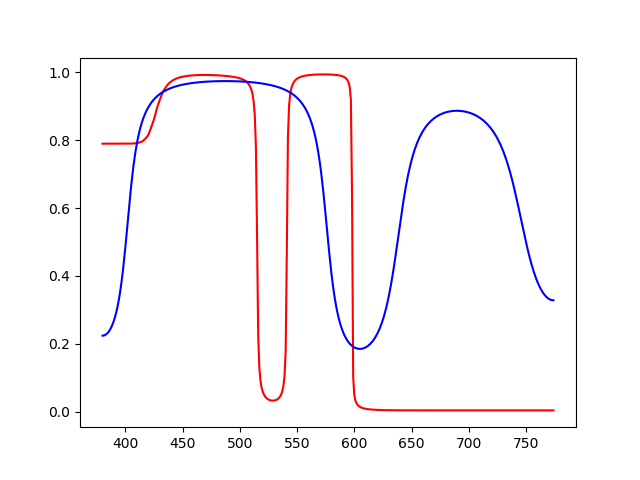
\includegraphics[width=\linewidth]{img/resultsTechniqueOpt_m5_cd32.png}
		\caption{$c=5, cd=32$,\\$RGB=(82.26, 172.74, 255)$,\\initial atlas = Page 14 from Munsell Book of Color}
		\label{fig:resultsTechniqueOpt_m5_cd32}
	\end{subfigure}
	\begin{subfigure}[t]{0.31\textwidth}
		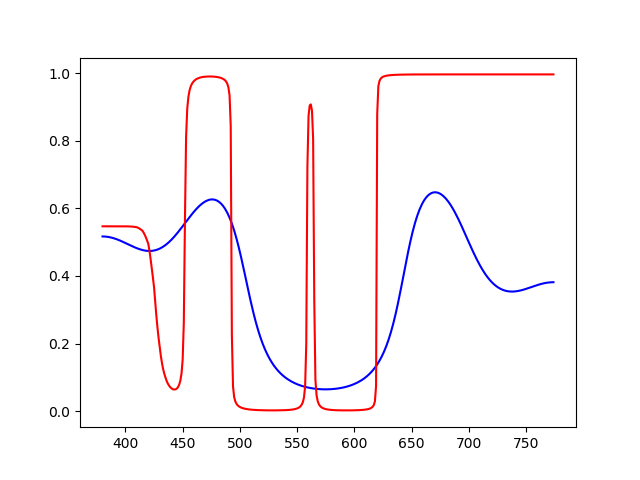
\includegraphics[width=\linewidth]{img/resultsTechniqueOpt_m7_cd16.png}
		\caption{$c=7, cd=16$,\\$RGB=(102, 17, 153)$,\\ fitted from middle}
		\label{fig:resultsTechniqueOpt_m7_cd16}
	\end{subfigure} 
	\caption{Comparison of warping and non-warping when used for fitting cubes, shown on cube entries from different cubes}
	\label{fig:resultsTechnique_optimizer}
\end{figure}

Obviously, the ideal solution would be to store the spectra with the method that provides better Delta E error and use non-warping for cube fitting afterwards. However, such an approach is impractical. Firstly, currently, as the first step of the spectral reconstruction is the conversion of wavelength array to a phase signal, using only one method means we can save this signal prior to fitting and reuse it, thus lowering time complexity. Using both methods would require either storing two phase signals, or recomputing them during each reconstruction. Secondly, as we use non-warping for cube fitting anyway, saving only some atlas entries with warping would be both impractical and would not provide too many benefits. Therefore, we leave the possibility of implementation of the support of both methods as future work.

\subsection{Cost functions} \label{ssec:costFunctions}

In addition to the moment storage technique, another thing greatly affecting the performance of the fitting are the cost functions of optimizer. Up until now, Borgtool has used three cost functions, or \emph{residuals}, for fitting with sigmoids, each of them specifying the absolute color difference in one axis of the RGB cube. Such an approach has outperformed both Euclidean color distance and even the Delta E difference --- the higher the number of meaningful residuals, the more information about the coefficients' behavior can the optimizer deduce, which, in turn, results in faster and more precise convergence to global optimum.

We therefore copy this approach to specify the color difference. In case of simple cube fitting with the user-specified number of moments (performed in step ref), the results obtained by such cost functions are satisfactory. However, a problem occurs upon fitting with atlas entries.

As already mentioned in ref, the process of seeding the cube with an atlas assigns each atlas entry its closest lattice point (atlas lattice point) in the cube. The distance between the atlas entry and its atlas lattice is dependent on the size of the voxel and, although it can be zero, the chances of that happening for every point of the atlas are slim. This implies that the points' curves cannot be exactly the same --- on the contrary, slight differences between them are even necessary.

The current cost functions, however, take into account the RGB differences only. They do not try to reconstruct similar shapes in any way, which, in turn, may result in significant shape errors in the resulting spectra. This behavior is not as perceivable in higher-dimensional cubes (e.g. 64), where the starting color difference is so low it does not allow the optimizer to change the reconstructed spectrum a lot before it converges. However, lower-dimensional cubes (e.g. 32) are prone to such behavior. Furthermore, as the specified coefficients are in their nature Fourier coefficients, the optimizer is apt to create spectra in the form of multiple waves with a rather high amplitude, which is only amplified the greater the color difference is.

\begin{figure}[t]
	\centering
	\captionsetup[subfigure]{font=footnotesize,labelfont=footnotesize}
	\captionsetup[subfigure]{justification=centering}
	\begin{subfigure}[t]{0.70\textwidth}
		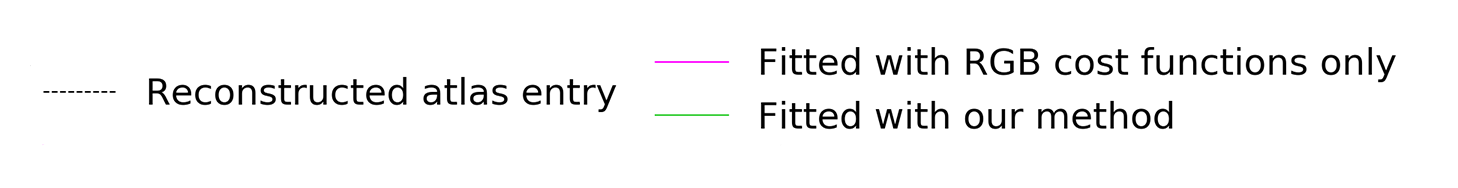
\includegraphics[width=\linewidth]{img/results_costFunctions_legend.png}
	\end{subfigure} \\
	\begin{subfigure}[t]{0.45\textwidth}
		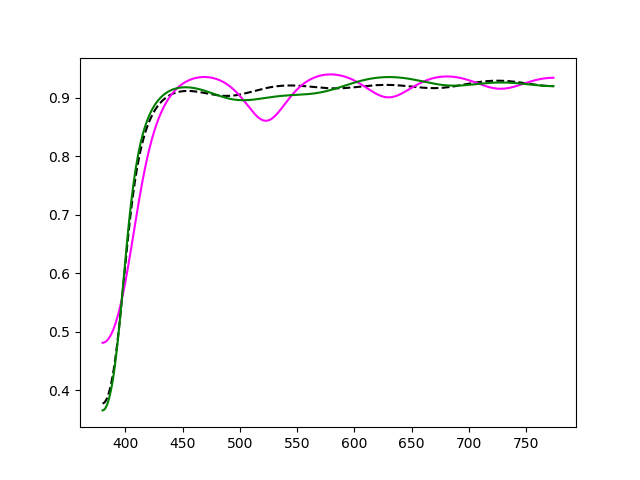
\includegraphics[width=\linewidth]{img/results_costFunctions_white_cd32.png}
		\caption{``white'' patch, CD = 32, $d = 5.81$}
		\label{fig:resultsCostFunctions_white32}
	\end{subfigure} \hspace{0.1em}
	\begin{subfigure}[t]{0.45\textwidth}
		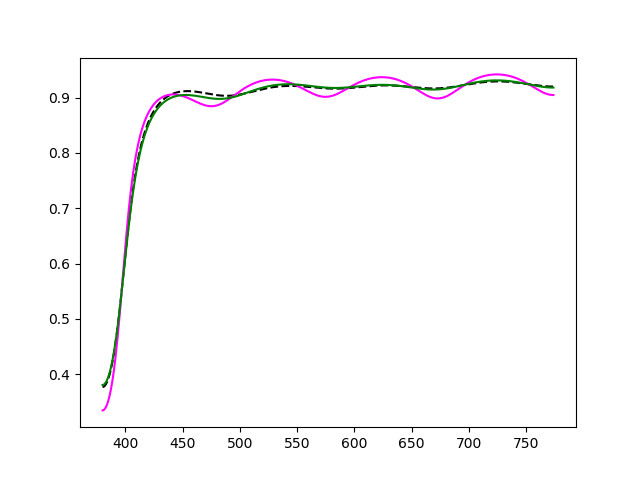
\includegraphics[width=\linewidth]{img/results_costFunctions_white_cd64.png}
		\caption{``white'' patch, CD = 64, $d = 1.99$}
		\label{fig:resultsCostFunctions_white64}
	\end{subfigure} \hspace{0.1em}
	\vspace{0.5em}\\
	\begin{subfigure}[t]{0.45\textwidth}
		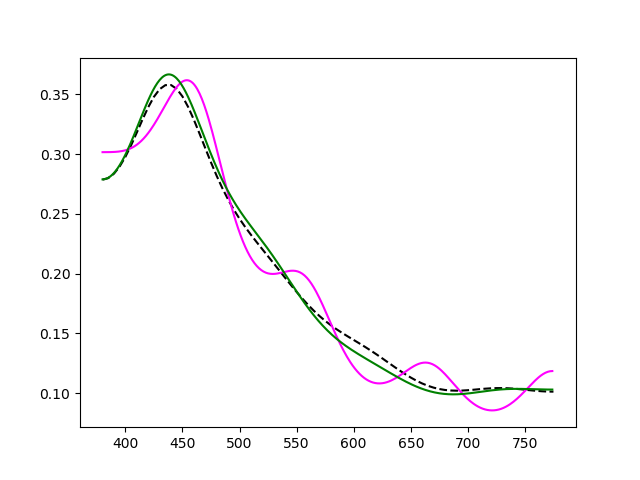
\includegraphics[width=\linewidth]{img/results_costFunctions_bs_cd32.png}
		\caption{``blue sky'' patch, CD = 32, $d = 4.1$}
		\label{fig:resultsCostFunctions_bs32}
	\end{subfigure} \hspace{0.1em}
	\begin{subfigure}[t]{0.45\textwidth}
		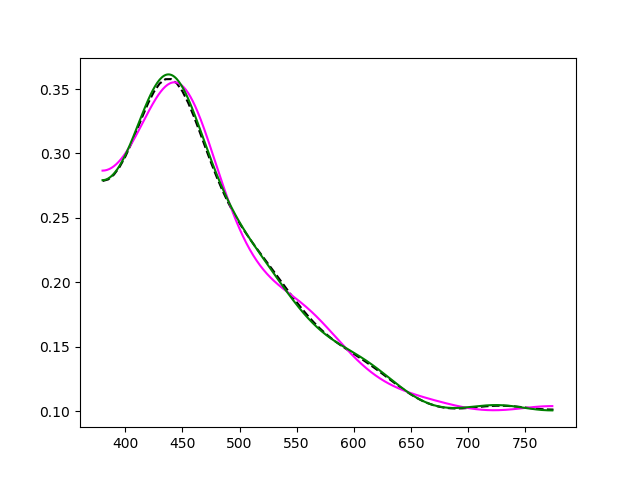
\includegraphics[width=\linewidth]{img/results_costFunctions_bs_cd64.png}
		\caption{``blue sky'' patch, CD = 64, $d = 0.96$}
		\label{fig:resultsCostFunctions_bs64}
	\end{subfigure}
	\caption{Comparison between the RGB cost functions and our method for fitting main atlas lattice points}
	\label{fig:resultsCostFunctions}
\end{figure}

We show an example of such behavior in~\cref{fig:resultsCostFunctions}, where we attempt to fit both the ``white'' and the ``blue sky'' patches of the Macbeth Color Checker to their main atlas lattice points in both a 32 and a 64-dimensional cube. The magenta plot represents the results of fitting with only the three cost functions, which is definitely undesired.

Note that we compare the optimized spectra not with the original atlas spectra, but with the spectra that is reconstructed from the original's coefficients. That way we can keep track of the optimizer's ability to mimic its input.

When fitting other spectral data, the optimizer does not behave as drastically as shown in~\cref{fig:resultsCostFunctions}. On the contrary, many fitted altas entries (such as the ``blue flower'' of the Macbeth Color Checker) resemble their input quite well. However, we must focus on the worst-case scenario as we do not wish to experience any metameric artifacts, not even in one color.

There are two ways of solving the presented problem --- either by simply using a higher-dimensional cube, or by adding cost functions that force the optimizer to keep the difference between the original and the reconstructed curve as low as possible.

We incline towards using more cost functions, both because the use of a higher-dimensional cube would require greater processing time, but also because the optimizer is prone to creating wave-like spectra nonetheless, even if the waves have much lower amplitude.

Our first idea was to add a fourth residual that would specify the least square error between the curves. Although the results with this method were quite satisfactory, the optimizer was sometimes prone to spikes, as the error was computed over the spectra as a whole rather. We therefore added one residual for each pair of spectral samples, which, in our case (as we sample with an increment of 1) sums up to roughly 400 cost functions. This allows the optimizer to specifically focus on the samples that it wants lowered, which therefore eliminates the possibility of spikes.

Although having this many residuals may seem far-fetched, the optimizer handles it well. It also does not reduce the importance of the three color cost functions. Its only notable issue is that it is prone to declaring optimization failures even if the residuals are satisfactory. This is due to its need to minimize all the residuals so they approach zero. However, we know that the original and resulting reflectance curves can not be exactly the same.

We solve this problem by adding a simple threshold to the optimizer. In case the least square error between one spectral sample pair is lower, the optimizer assumes it to be zero and is not concerned by it anymore. Initially, we set the threshold to zero, but increase it if the optimizer fails and try again. 

The heuristic regarding the threshold does not, on average, need to be invoked more than 2-3 times when fitting an arbitrary atlas to a sufficiently-sized cube (i.e. 64-dimensional). It is clear that by lowering the cube's dimension, the heuristic becomes more utilized. For example, for an 8-dimensional cube, it reaches up to 100 invocations, and even then the fitting may not always be successful.

We, however, do not concern ourselves much with cubes of such low dimension --- even for a 32-dimensional cube, the difference between an atlas lattice point and an atlas entry can be as much as $d = 13.86$ (in which $d$ denotes the Euclidean distance), which already suggests a rather significant difference between reflectance spectra and therefore implies loss of atlas information. We therefore strongly recommend the user to avoid cubes of low dimensions (i.e. under 32).

In~\cref{fig:resultsCostFunctions}, we provide a comparison between the results obtained with our cost functions and the results obtained with the original ones. It is clear that our approach is superior in terms of spectral shape and, as the implementation of the color specifying residuals is identical in both approaches, the resulting RGB values are extremely similar. We therefore use our newly presented residuals for atlas fitting.

Our cost functions give us the ability to control the shape of the resulting spectra. By further utilizing them, we could fit the neighbors of atlas lattice points so that their spectra is extremely similar. Applying this method to the whole cube-fitting process could therefore create an uplifting model with a rather uniform spectra. Such an uplifting model is especially desired for the interpolation phase in rendering.

However, two problems already arise with this approach. Firstly, by growing the cube from multiple atlas entries at the same time, there is bound to be a point in which neighbors are fitted from different prior atlas entries. By our premise, this would mean that the spectra of these two points could be vastly different.

Another issue is the significant increase in time complexity. Even excluding the complex calculations the optimizer must perform during minimization, the computation of around 400 residuals takes a lot more time than just computing the original 3. The process of fitting a 32-dimensional cube, regardless of the number of its moments and the allowed optimizer's threshold, then takes hours instead of mere minutes when executed on an ordinary desktop PC. This renders our cost functions unusable for cube fitting and we must therefore settle for using the RGB cost functions only.

The increased time complexity gives rise to the question of whether it is even feasible to use our cost functions for atlas fitting. It is true that in some cases, for example when seeding with the Munsell Color Atlas, in which the atlas lattice points make up a significant portion of the cube, the time difference is noticeable. However, if we wish to seed the cube with all the atlas entries, we often require a cube of a much higher dimension, the fitting of which diminishes the time importance of the initial atlas fit. Although this may not be true in all cases (e.g. we could create an atlas the size of the cube with each entry mapping to a different lattice point), it is still beneficial to trade off the possibility of a higher time complexity for much precise spectra.

Therefore, we use the original RGB difference cost functions for fitting regular point and our new cost functions for fitting atlas lattice point.

\subsection{Number of moments}
 
Maybe add a section about unfittable cubes?

However, correct round-trips are not the only factor we need to take into consideration when fitting the cube. We also need to focus on both the \emph{smoothness of the resulting spectra} and the \emph{behavior of the optimizer} under the current technique.

The smoothness of the spectra is especially important for the interpolation process that takes place during the rendering. Interpolating multiple spiky, non-similar spectra would result in similarly uneven spectra, which, in addition to incorrect color, may be susceptible to extreme metameric artifacts.  

The behavior of the optimizer also plays a big role. During the optimization, it takes into account only the resulting RGB of the curve rather than the shape of the curve itself. Therefore, it does not aim for a curve with a similar shape than its neighbor, which may likewise cause issues during the interpolation.

When we fit from the middle, we only aim for the smoothness of the resulting spectra and for the behavior of the optimizer. We therefore want as less coefficients as possible and, as we do not care about round trips, we can use any of the techniques available.

We already said that using 9 coefficients is unecessary, as 3 already create rather smooth spectra that is way better for interpolation. However, we here find out that it is not only unnecessary but extremely discouraged. We can see in the image how the fitting proceeds. It amplifies the already existing wave-like patterns, exhibiting the same behavior as it did during atlas fitting, which is caused by the cost functions not considering the shape of the resulting spectra. By allowing only three coefficients, we limit the optimizer so it must create smooth spectra and it cannot create crazy shapes. Additionaly, it is better for performance - fiting of a 9-coefficients takes around blabla, while fitting 3 takes blabla. We provide measurements here? of performance

Although we cannot control shape, we can control smoothness. We want smooth spectra both for interpolation purposes and because smooth spectra is less prone to metameric artifacts, see chapter 1.

The behavior we talked about before of the optimizer is a problem 
It would be extremely beneficial for the

For middle fitting, we always recommend 2 moments, 3 coeffs due to the runtime. Moreover, they are very smooth but not straight which is ideal for our purposes. Obviously, we can fit with higher but that takes a lot of time and does not provide any advantage. The default setting is therefore 3 coefs, 2 moments.

Obviously, fitting with these causes metameric artifacts, similar to the ones created by sigmoid, we show these in PICTURE. We can also show metameric artifacts when fitting with more? (try this maybe)

Another slight trick is to use a lower number of coefficients - we therefore do not get as big artifacts because we cannot possibly reconstruct such crazy spectra with low number of coefficients. 

The optimizer is always faster for lower number of coefficients as it does not need to change them up as much. Also faster but does not change them so much SO it results in spectrum that is similar to the first one. However, we cannot possibly simulate the curve with only the limited number of coefficients, the table says so. Therefore we must find something in the middle. We try not to focus on performance here because obviously, fitting anything that is higher than 32 takes hours and we want to have it look the best way we can.

\section{Performace}

heuristics performance, overall runtime of the cube

\section{Rendering}

- which technique gives the best results (metamerism results)


Also mention that it is multi-threaded and performance is not really a priority - the cube has to be created only once and then can be reused as much as the artists need.
